\documentclass[10pt]{article}
\usepackage{amsmath, amssymb}
\usepackage{graphicx}

\begin{document}

\begin{center}
    \LARGE {Problem Set 2 – Shallow and Deep Networks} \\[1em]
    \Large{DS542 – DL4DS} \\[0.5em]
    \large Spring, 2025 \\
    \large Sicheng Yi
\end{center}

\vspace{2em}

\noindent\textbf{Note:} Refer to the equations in the \textit{Understanding Deep Learning} textbook to solve the following problems.

\vspace{2em}

\section*{Problem 3.2}
For each of the four linear regions in Figure 3.3j, indicate which hidden units are inactive and which are active (i.e., which do and do not clip their inputs).

\begin{figure}[h]
    \centering
    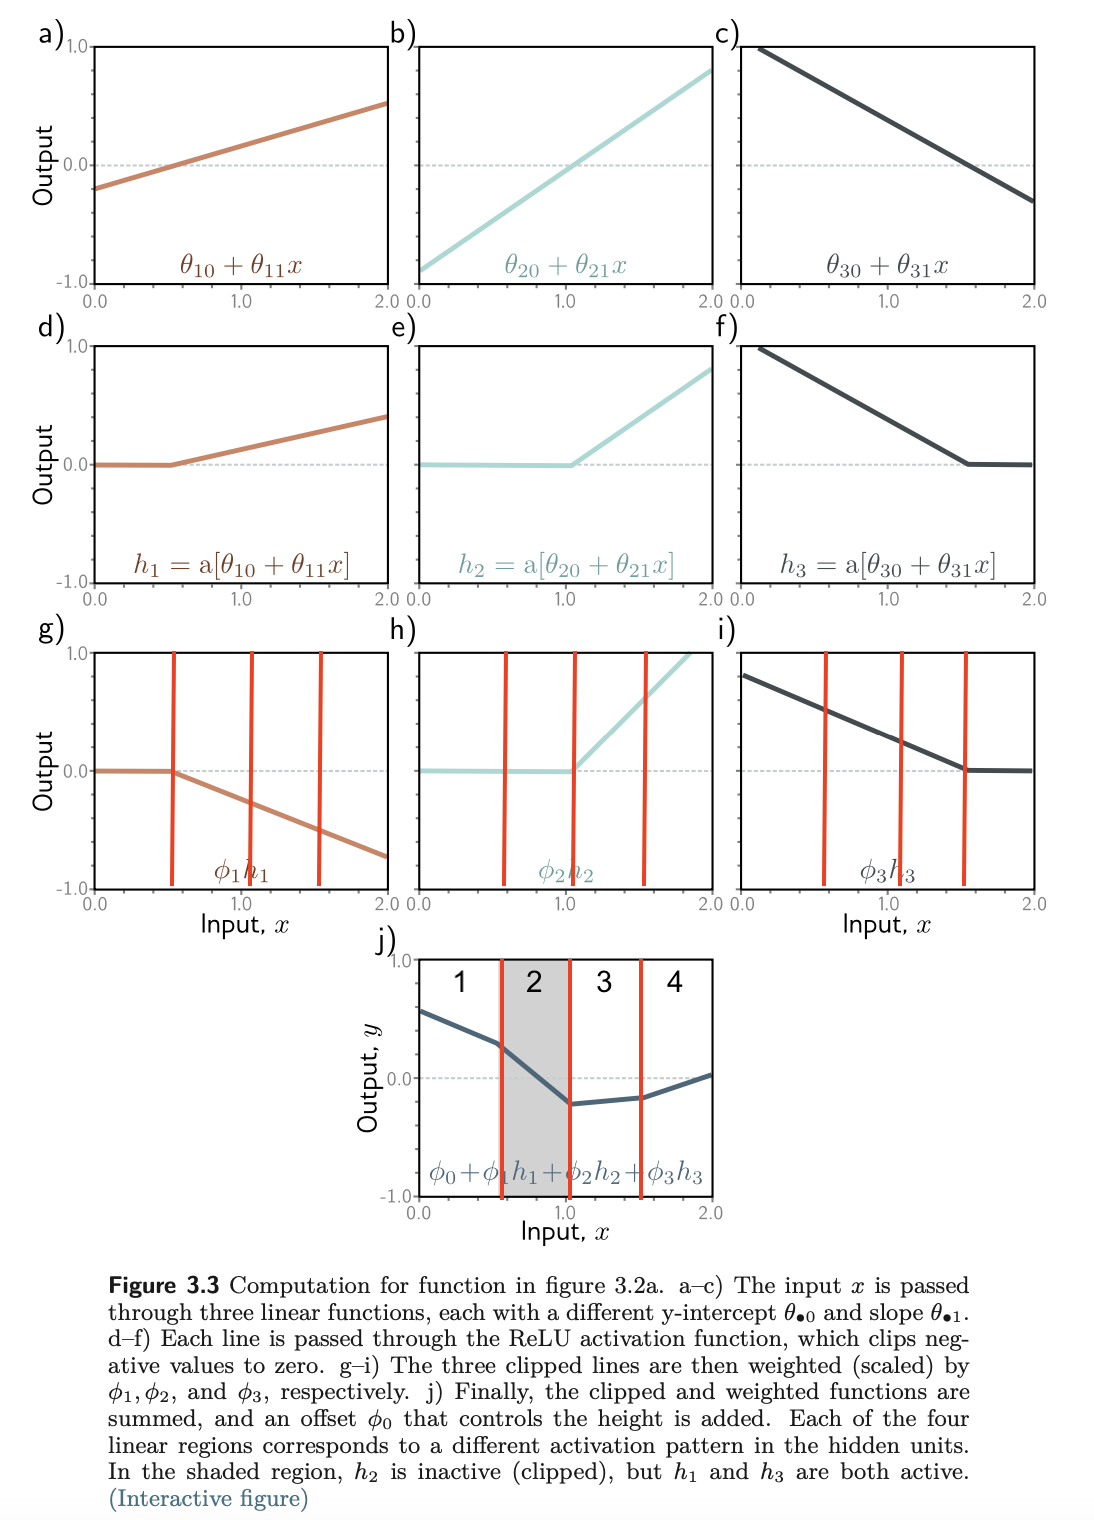
\includegraphics[width=1\textwidth]{image.png}
    \caption{problem 3.2}
    \label{fig:problem32}
\end{figure}

\ 

\noindent Answer: Refer to Figure~\ref{fig:problem32} at the end

\noindent Region 1: only h3 (i) is activated 

\noindent Region 2: h1 (g) and h3 (i) are activated
 
\noindent Region 3: h1 (g), h2 (h), and h3 (i) are all activated

\noindent Region 4: h1 (g) and h2 (h) are activated



\vspace{2em}

\section*{Problem 3.5}

Prove that the following property holds for $\alpha \in \mathbb{R}^+$:
\[
\text{ReLU}[\alpha \cdot z] = \alpha \cdot \text{ReLU}[z].
\]
This is known as the non-negative homogeneity property of the ReLU function.

\ 

\noindent Answer:

\noindent ReLu is 0 when input z is negative, otherwise z when non-negative. 

$$ ReLU[z] = \max(0, z) $$

$$ ReLU[a \cdot z] = \max(0a , az) = a \max(0, z)  $$

$$ ReLU[a \cdot z] = a ReLU[z] $$ 





\vspace{2em}

\section*{Problem 4.6}

Consider a network with $D_i = 1$ input, $D_o = 1$ output, $K = 10$ layers, and $D = 10$ hidden units in each. Would the number of weights increase more -- if we increased the depth by one or the width by one? Provide your reasoning.



\ 

\noindent Answer:

\noindent  Input: $D_i = 1$, Output: $D_o = 1$,

\noindent Layers: $K = 10$, 9 transitions between each hidden layers

\noindent  Hidden Units in each layer : $D = 10$

\ 

\noindent Total Parameters $ n = 10 + 10 \times 10 \times 9 + 10 = 920  $, if not including the bias terms

\ 

\noindent Increase depth by 1, 11 layers in total, 10 transitions between each hidden layers

\noindent Total Parameters $ n = 10 + 10 \times 10 \times 10 + 10 = 1020 $, if not including the bias terms

\noindent Increase of weights is $1020-920=100$

\ 

\noindent Increase width by 1, each layer now has 11 hidden units 

\noindent Total Parameters $ n = 11 + 11 \times 11 \times 9  + 11 = 1111 $, if not including the bias terms

\noindent Increase of weights is $1111-920=191$

\ 

\noindent $100 < 191$, depth < width

\noindent  Therefore, number of weights will increase more if increase width by 1, over increase depth by 1. 


\end{document}
